\chapter{Casos de uso}

%=====================================================

\section{Diagramas de Caso de uso}

\begin{figure}[!htb]
\centering
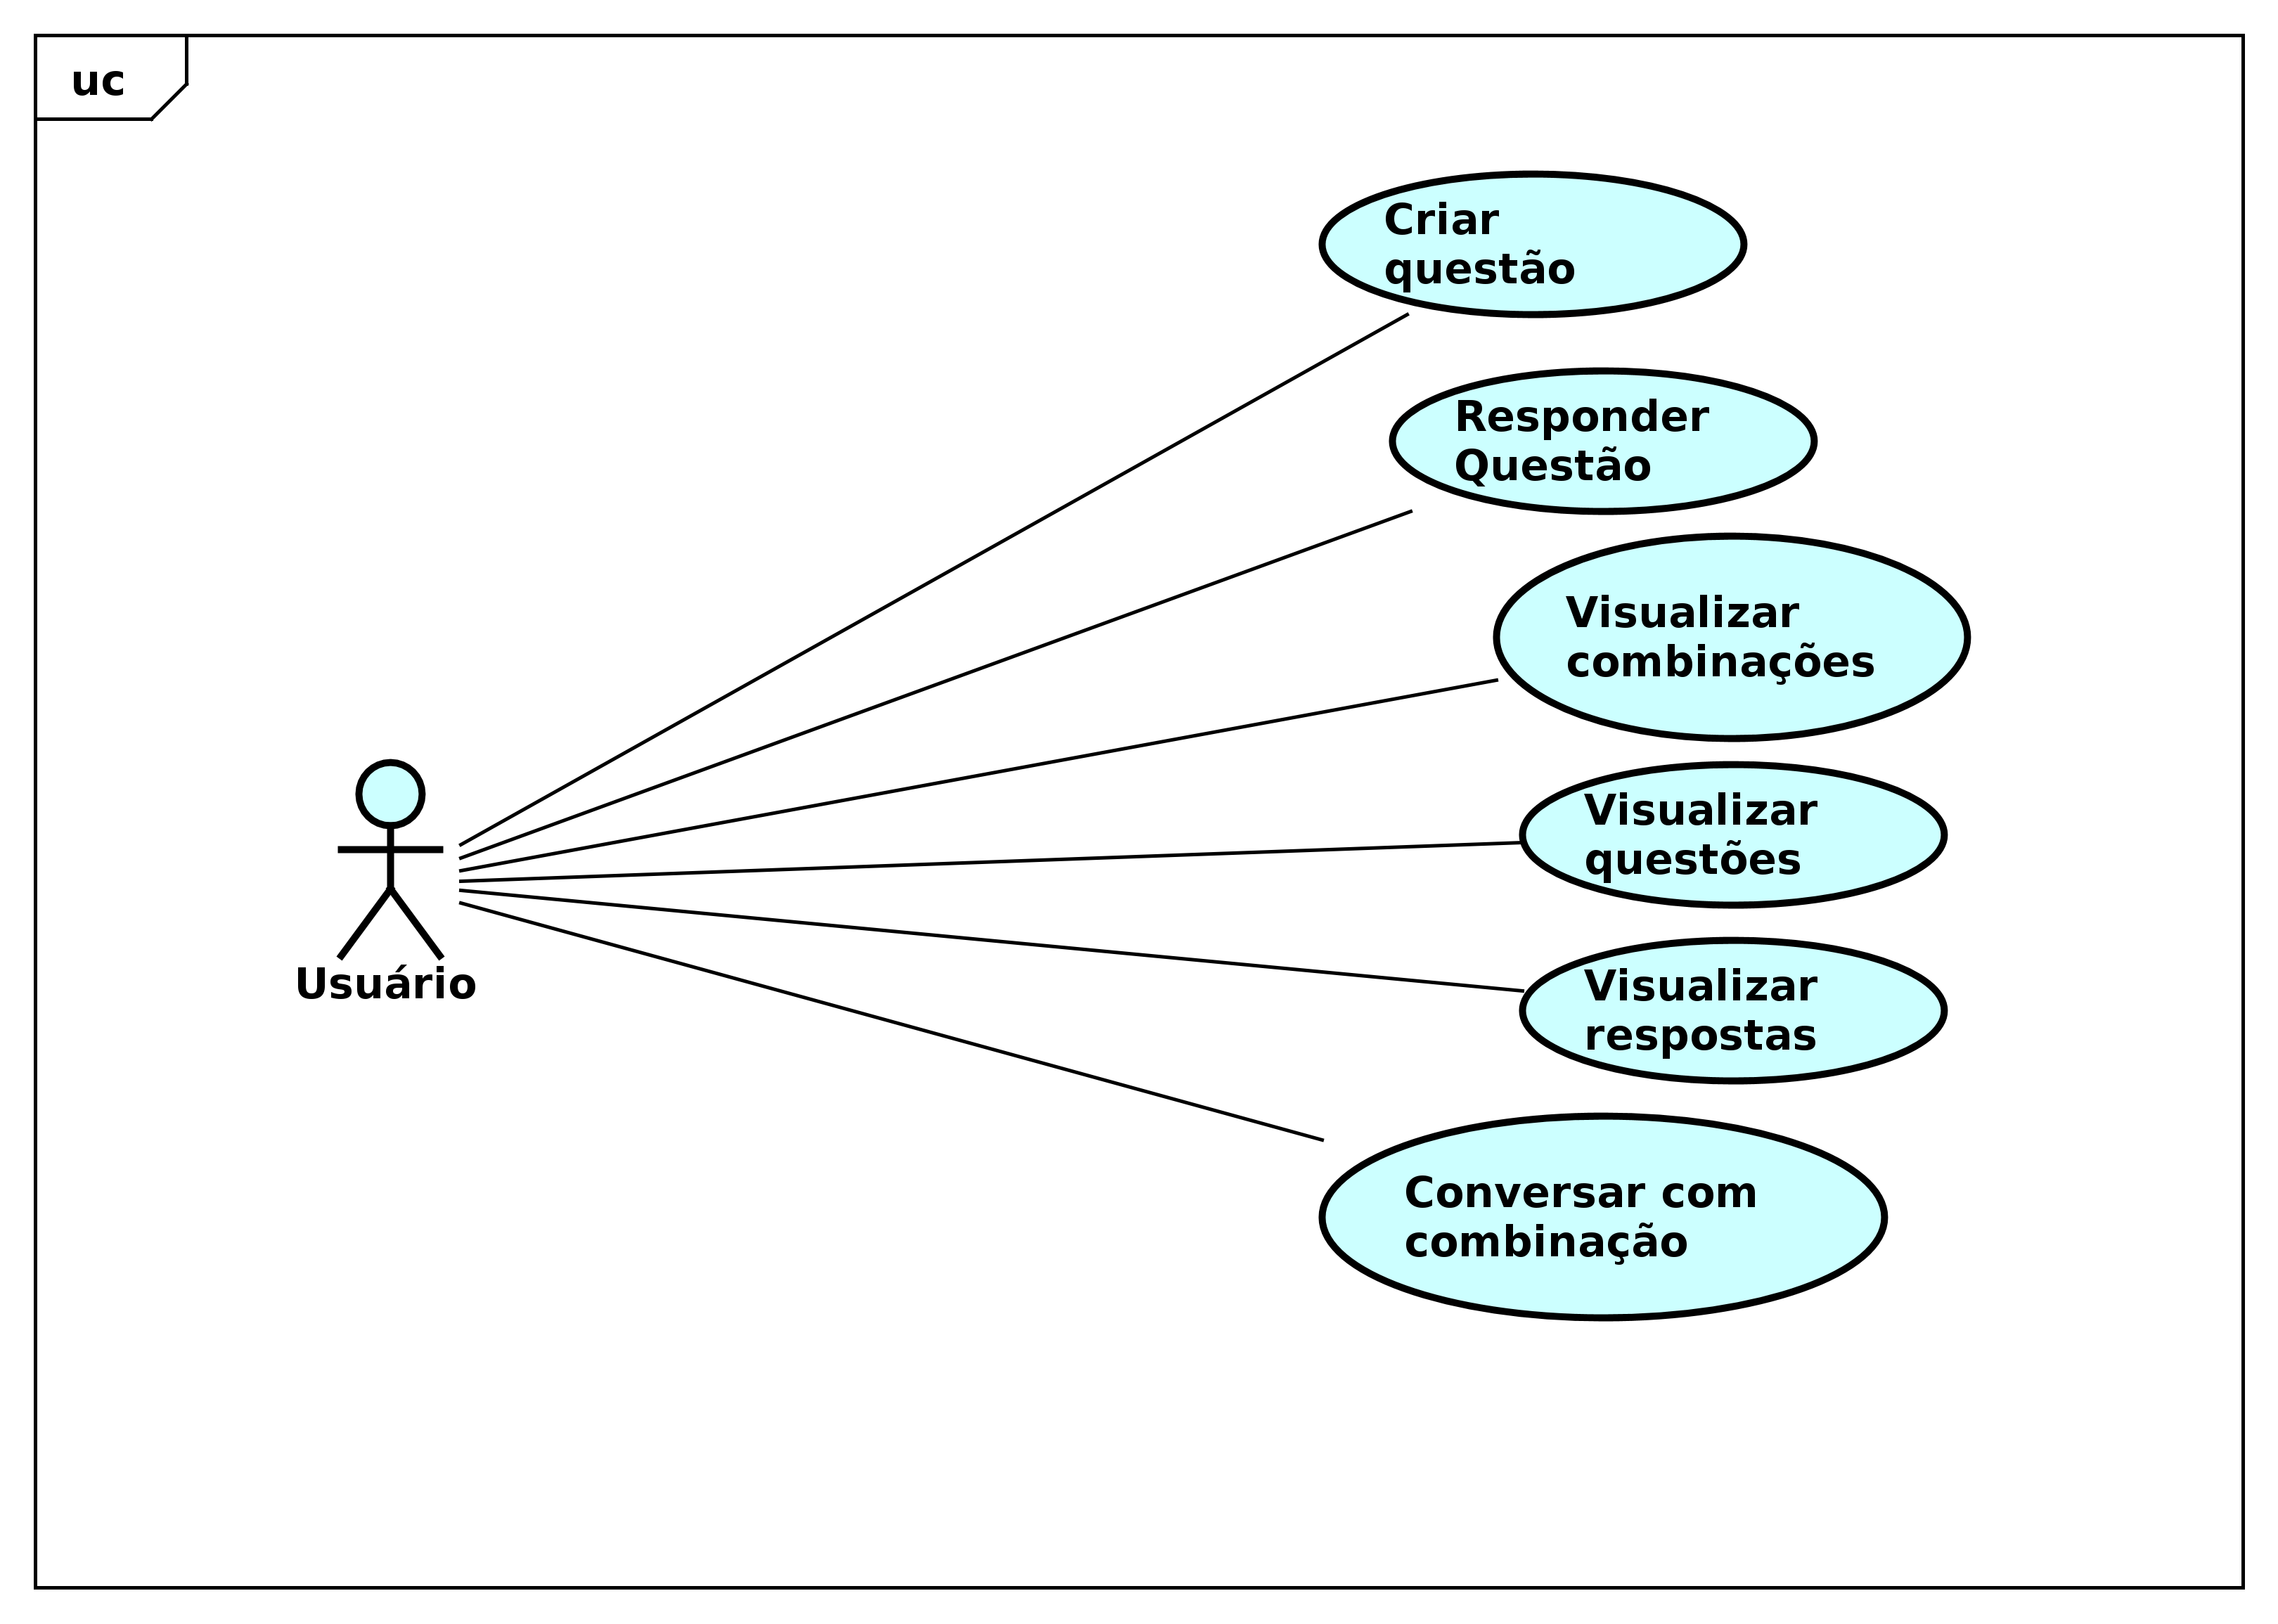
\includegraphics[width=16cm]{DCU1.png}
\caption{Diagrama de caso de uso nível 1. Fonte: os autores.}
\label{fig:DCU1}
\end{figure}

\begin{figure}[!htb]
\centering
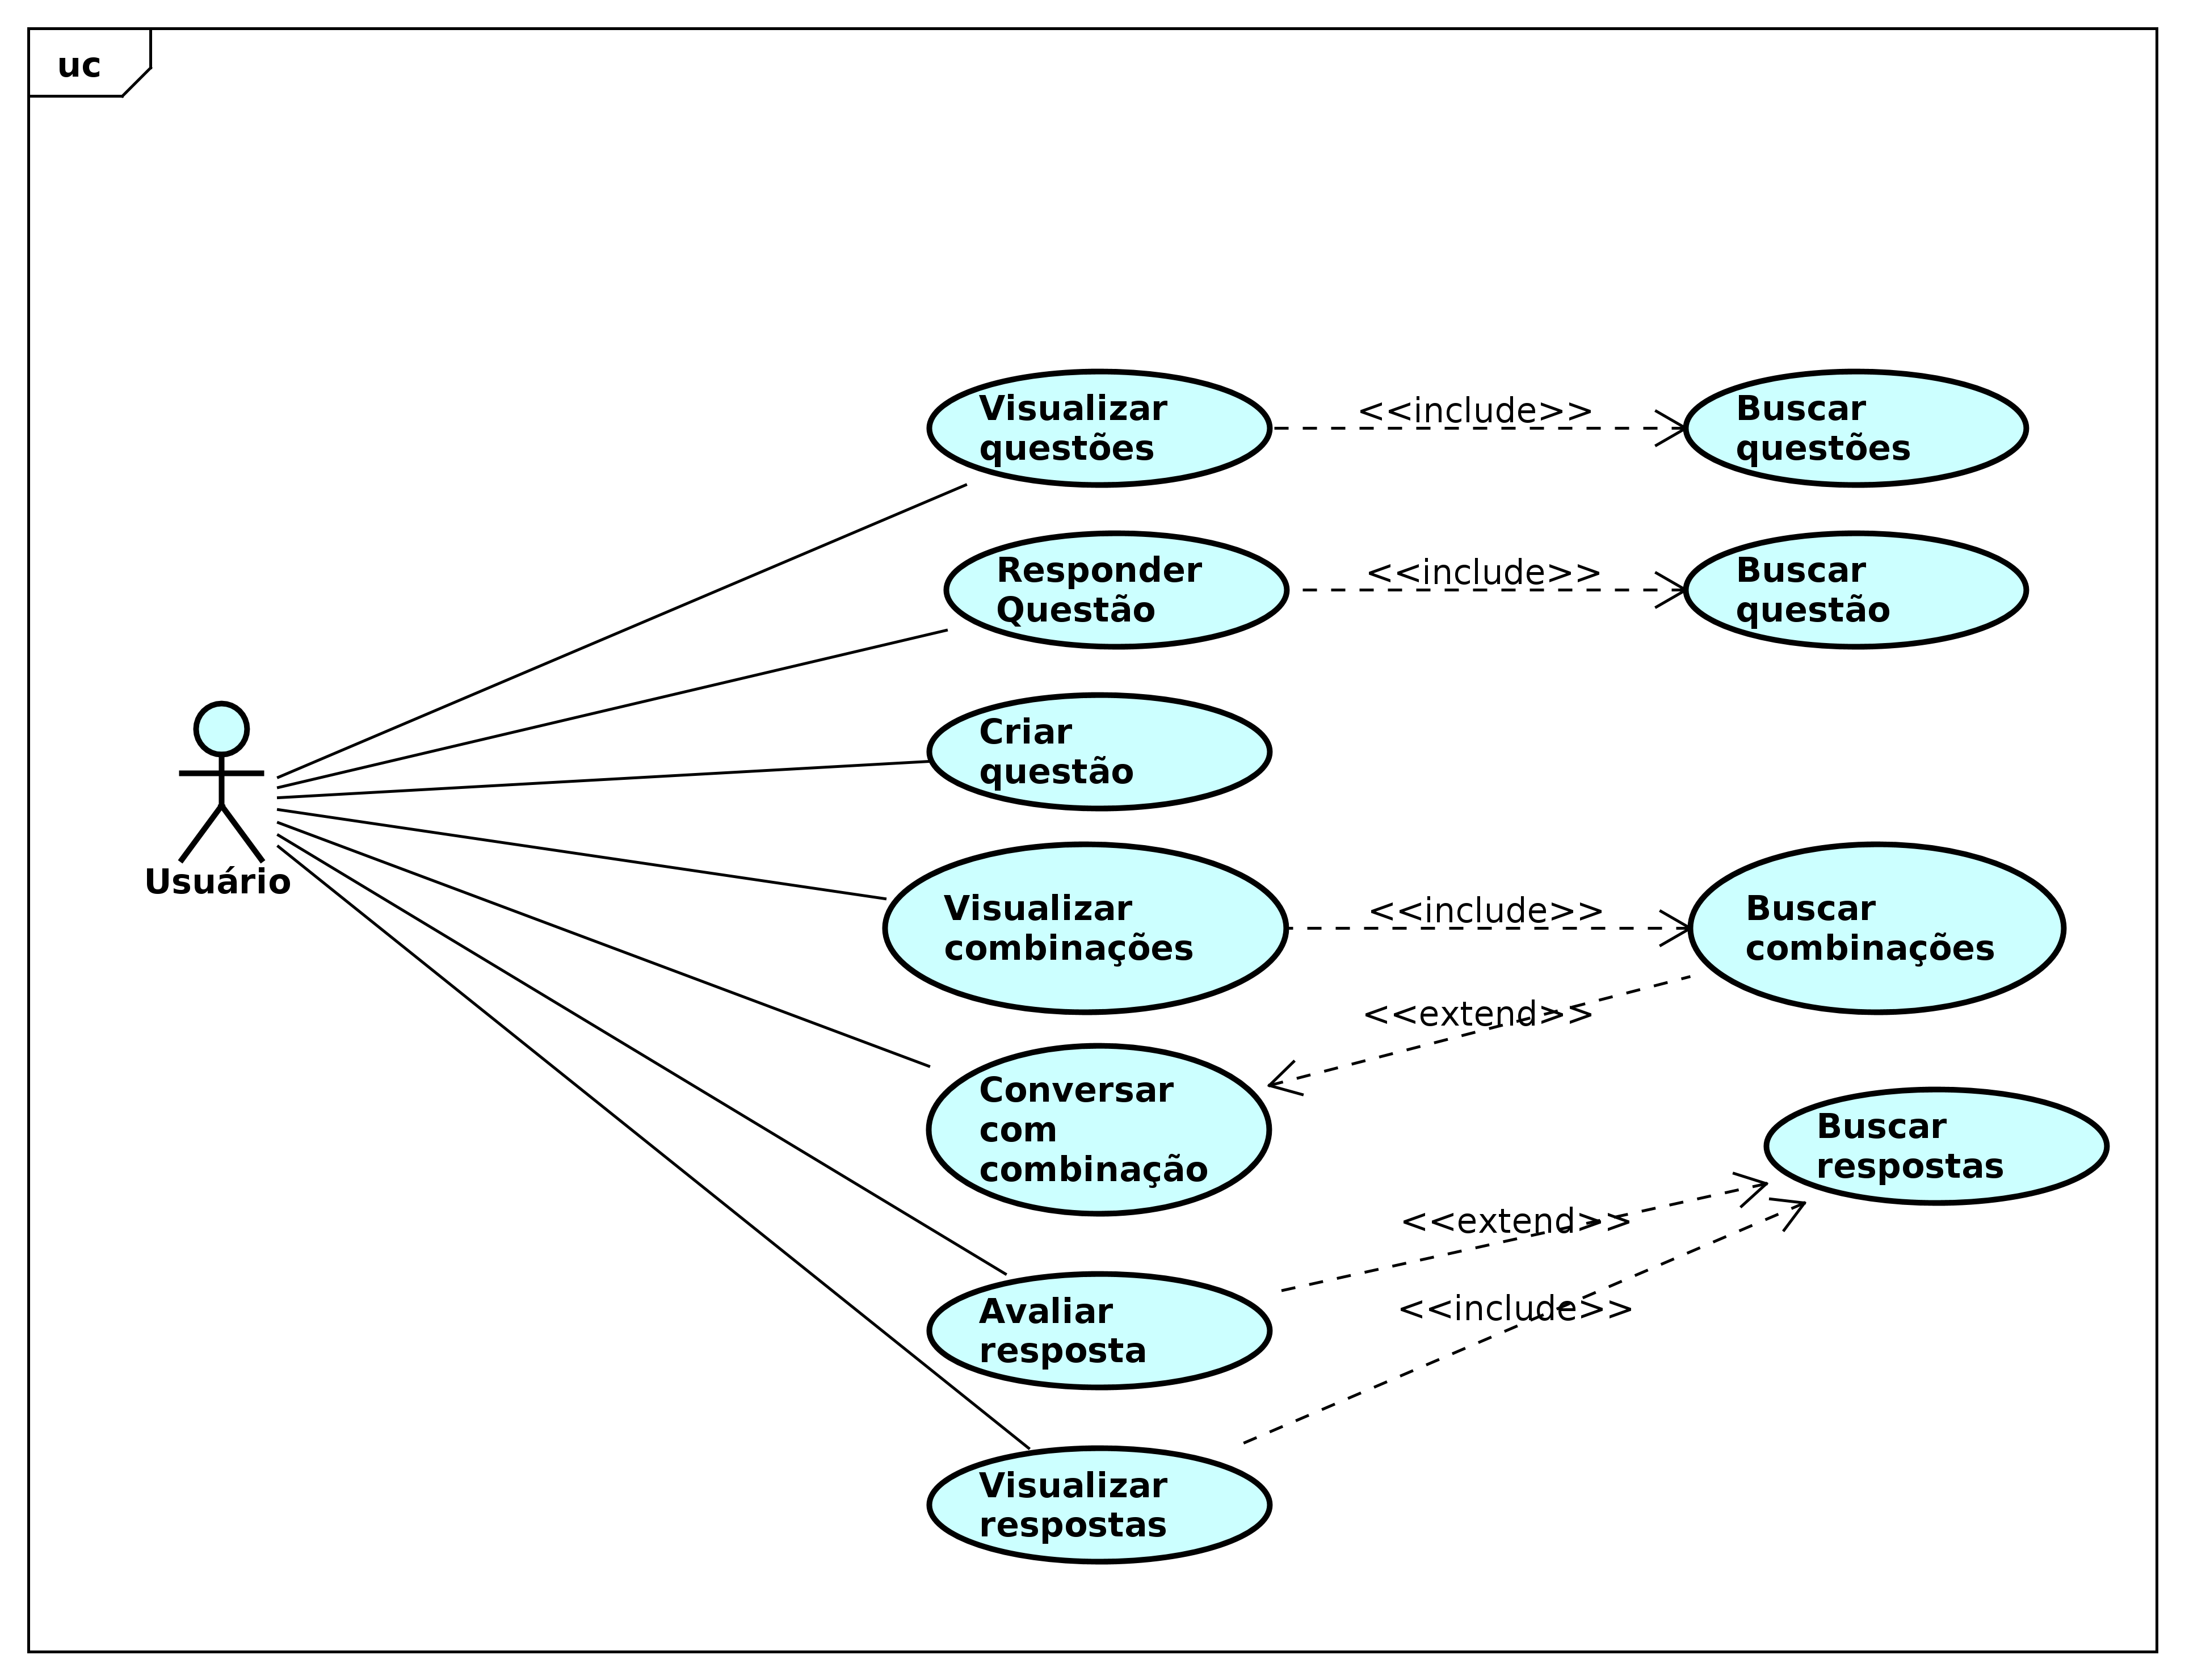
\includegraphics[width=16cm]{DCU2.png}
\caption{Diagrama de caso de uso nível 2. Fonte: os autores.}
\label{fig:DCU2}
\end{figure}
%=====================================================

\section{Diagramas de sequência}

\begin{figure}[!htb]
\centering
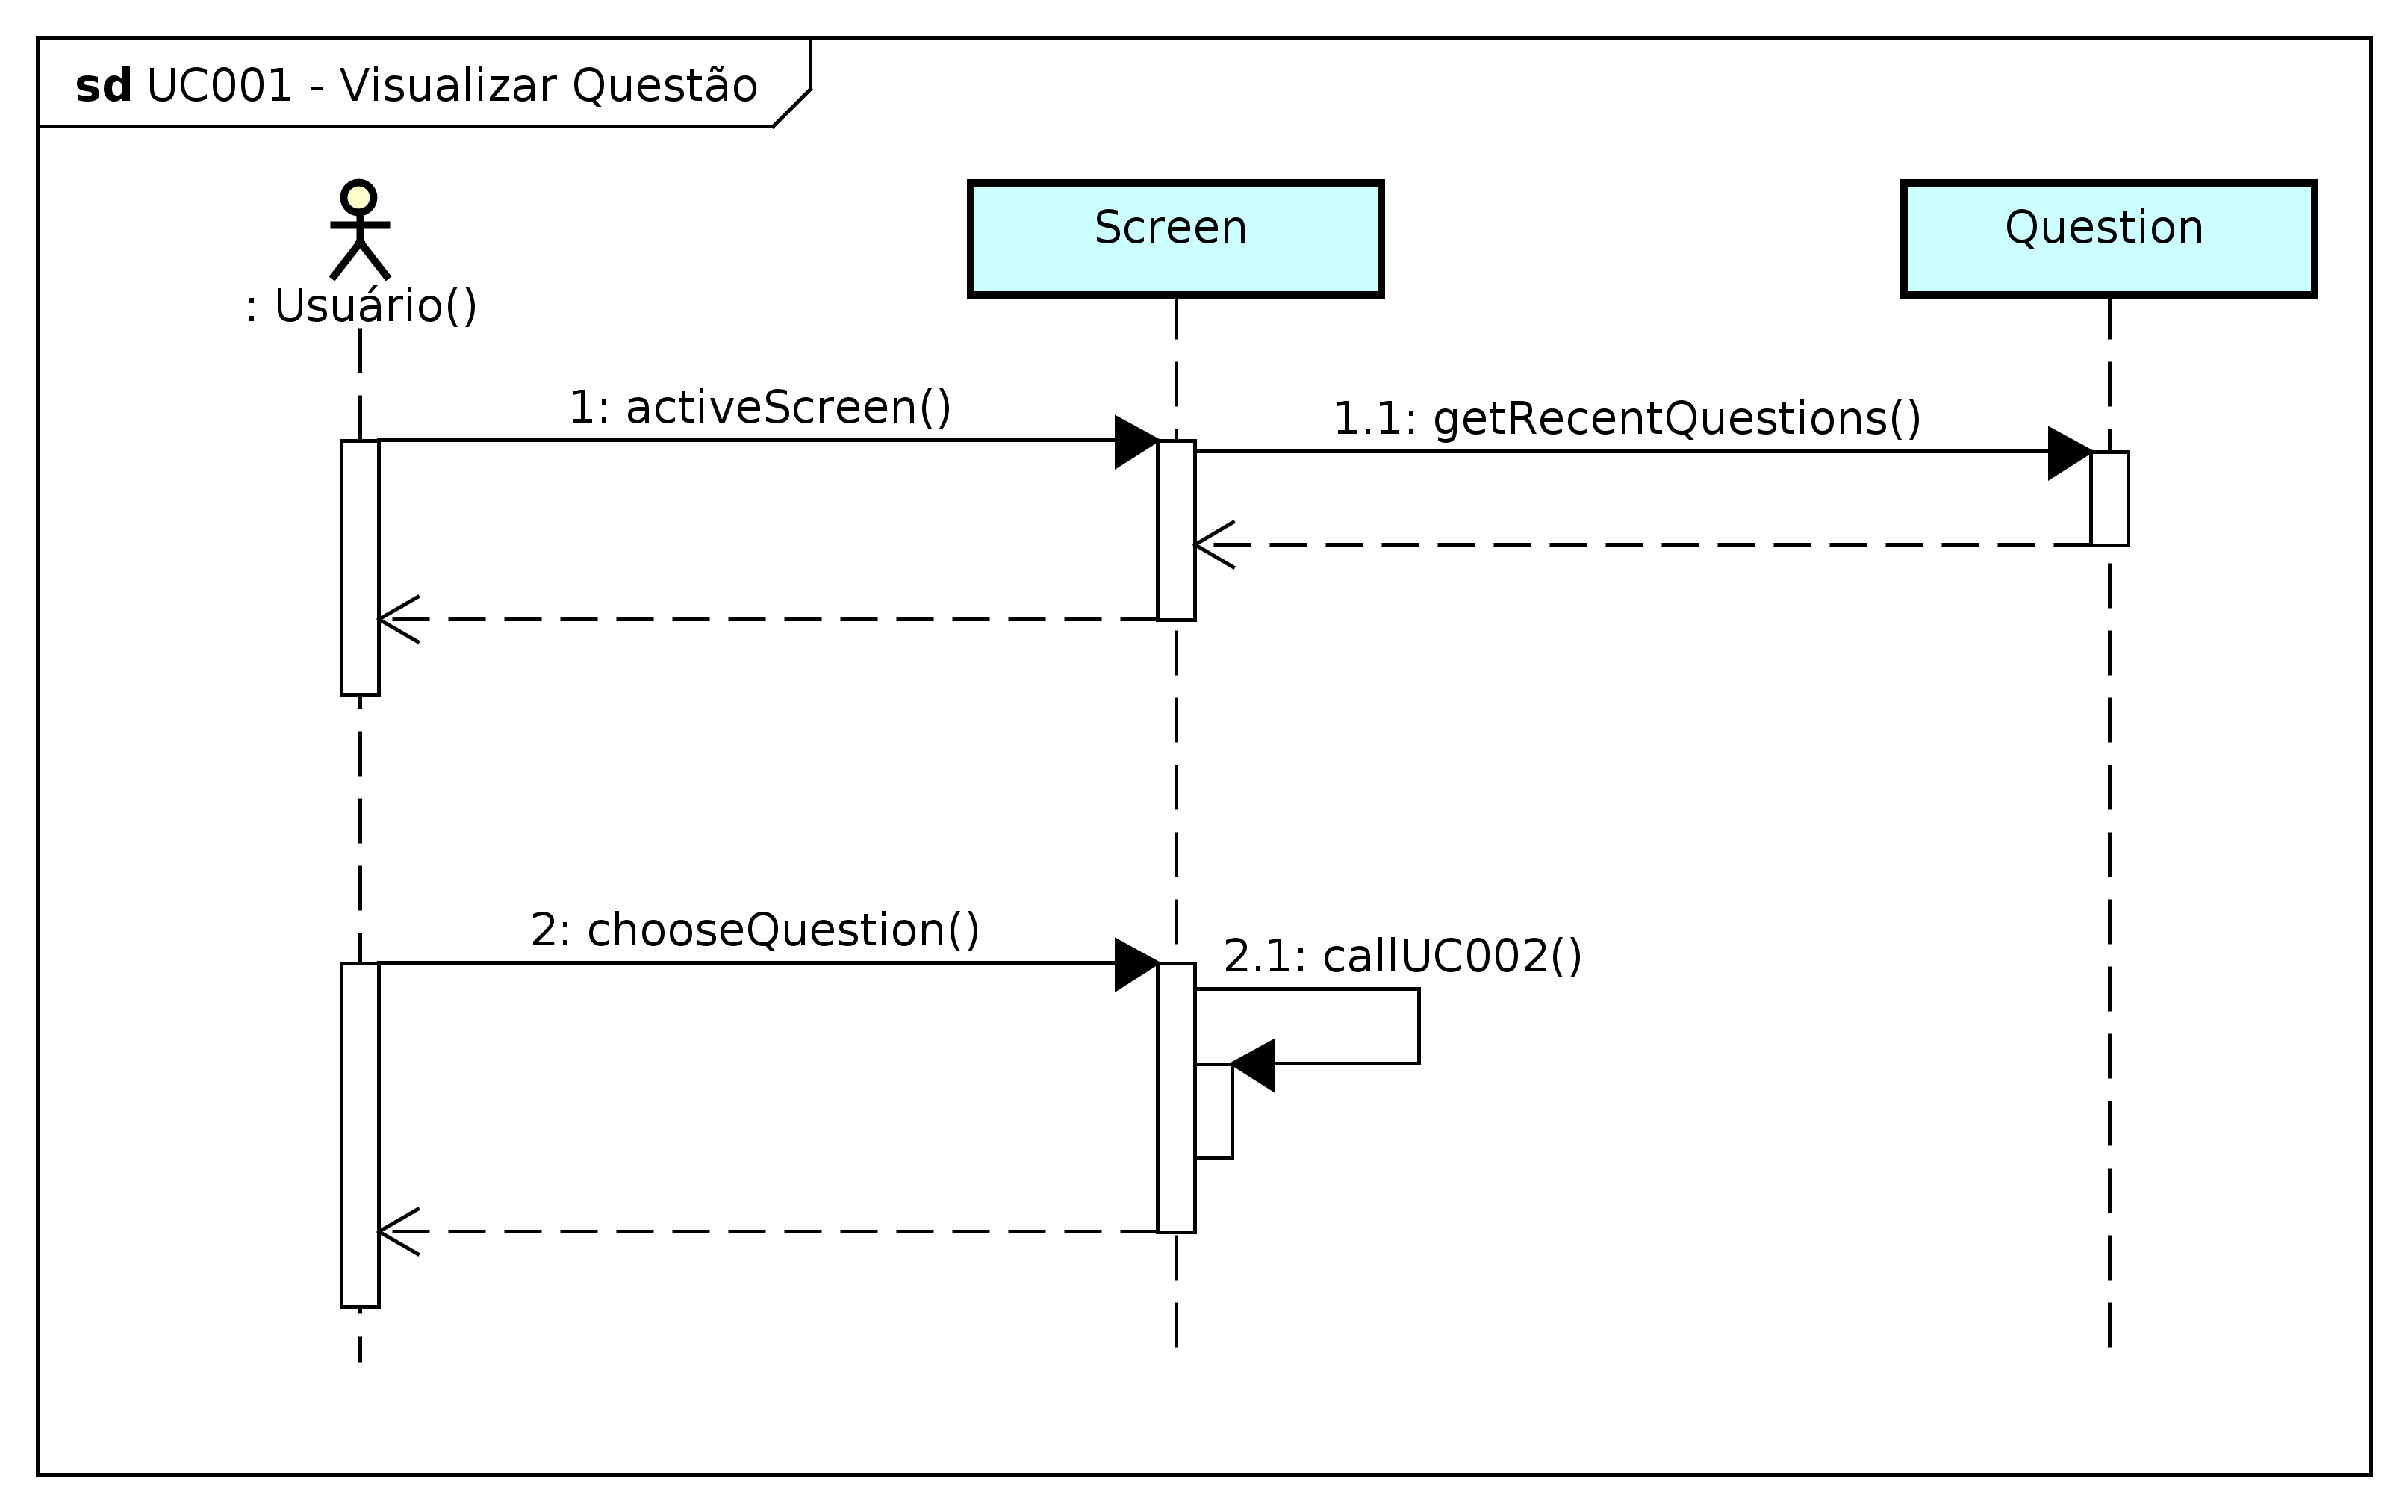
\includegraphics[width=16cm]{UC001-VisualizarQuestao.png}
\caption{Diagrama de caso de uso UC001 - Visualizar Questão. Fonte: os autores.}
\label{fig:UC001}
\end{figure}

\begin{figure}[!htb]
\centering
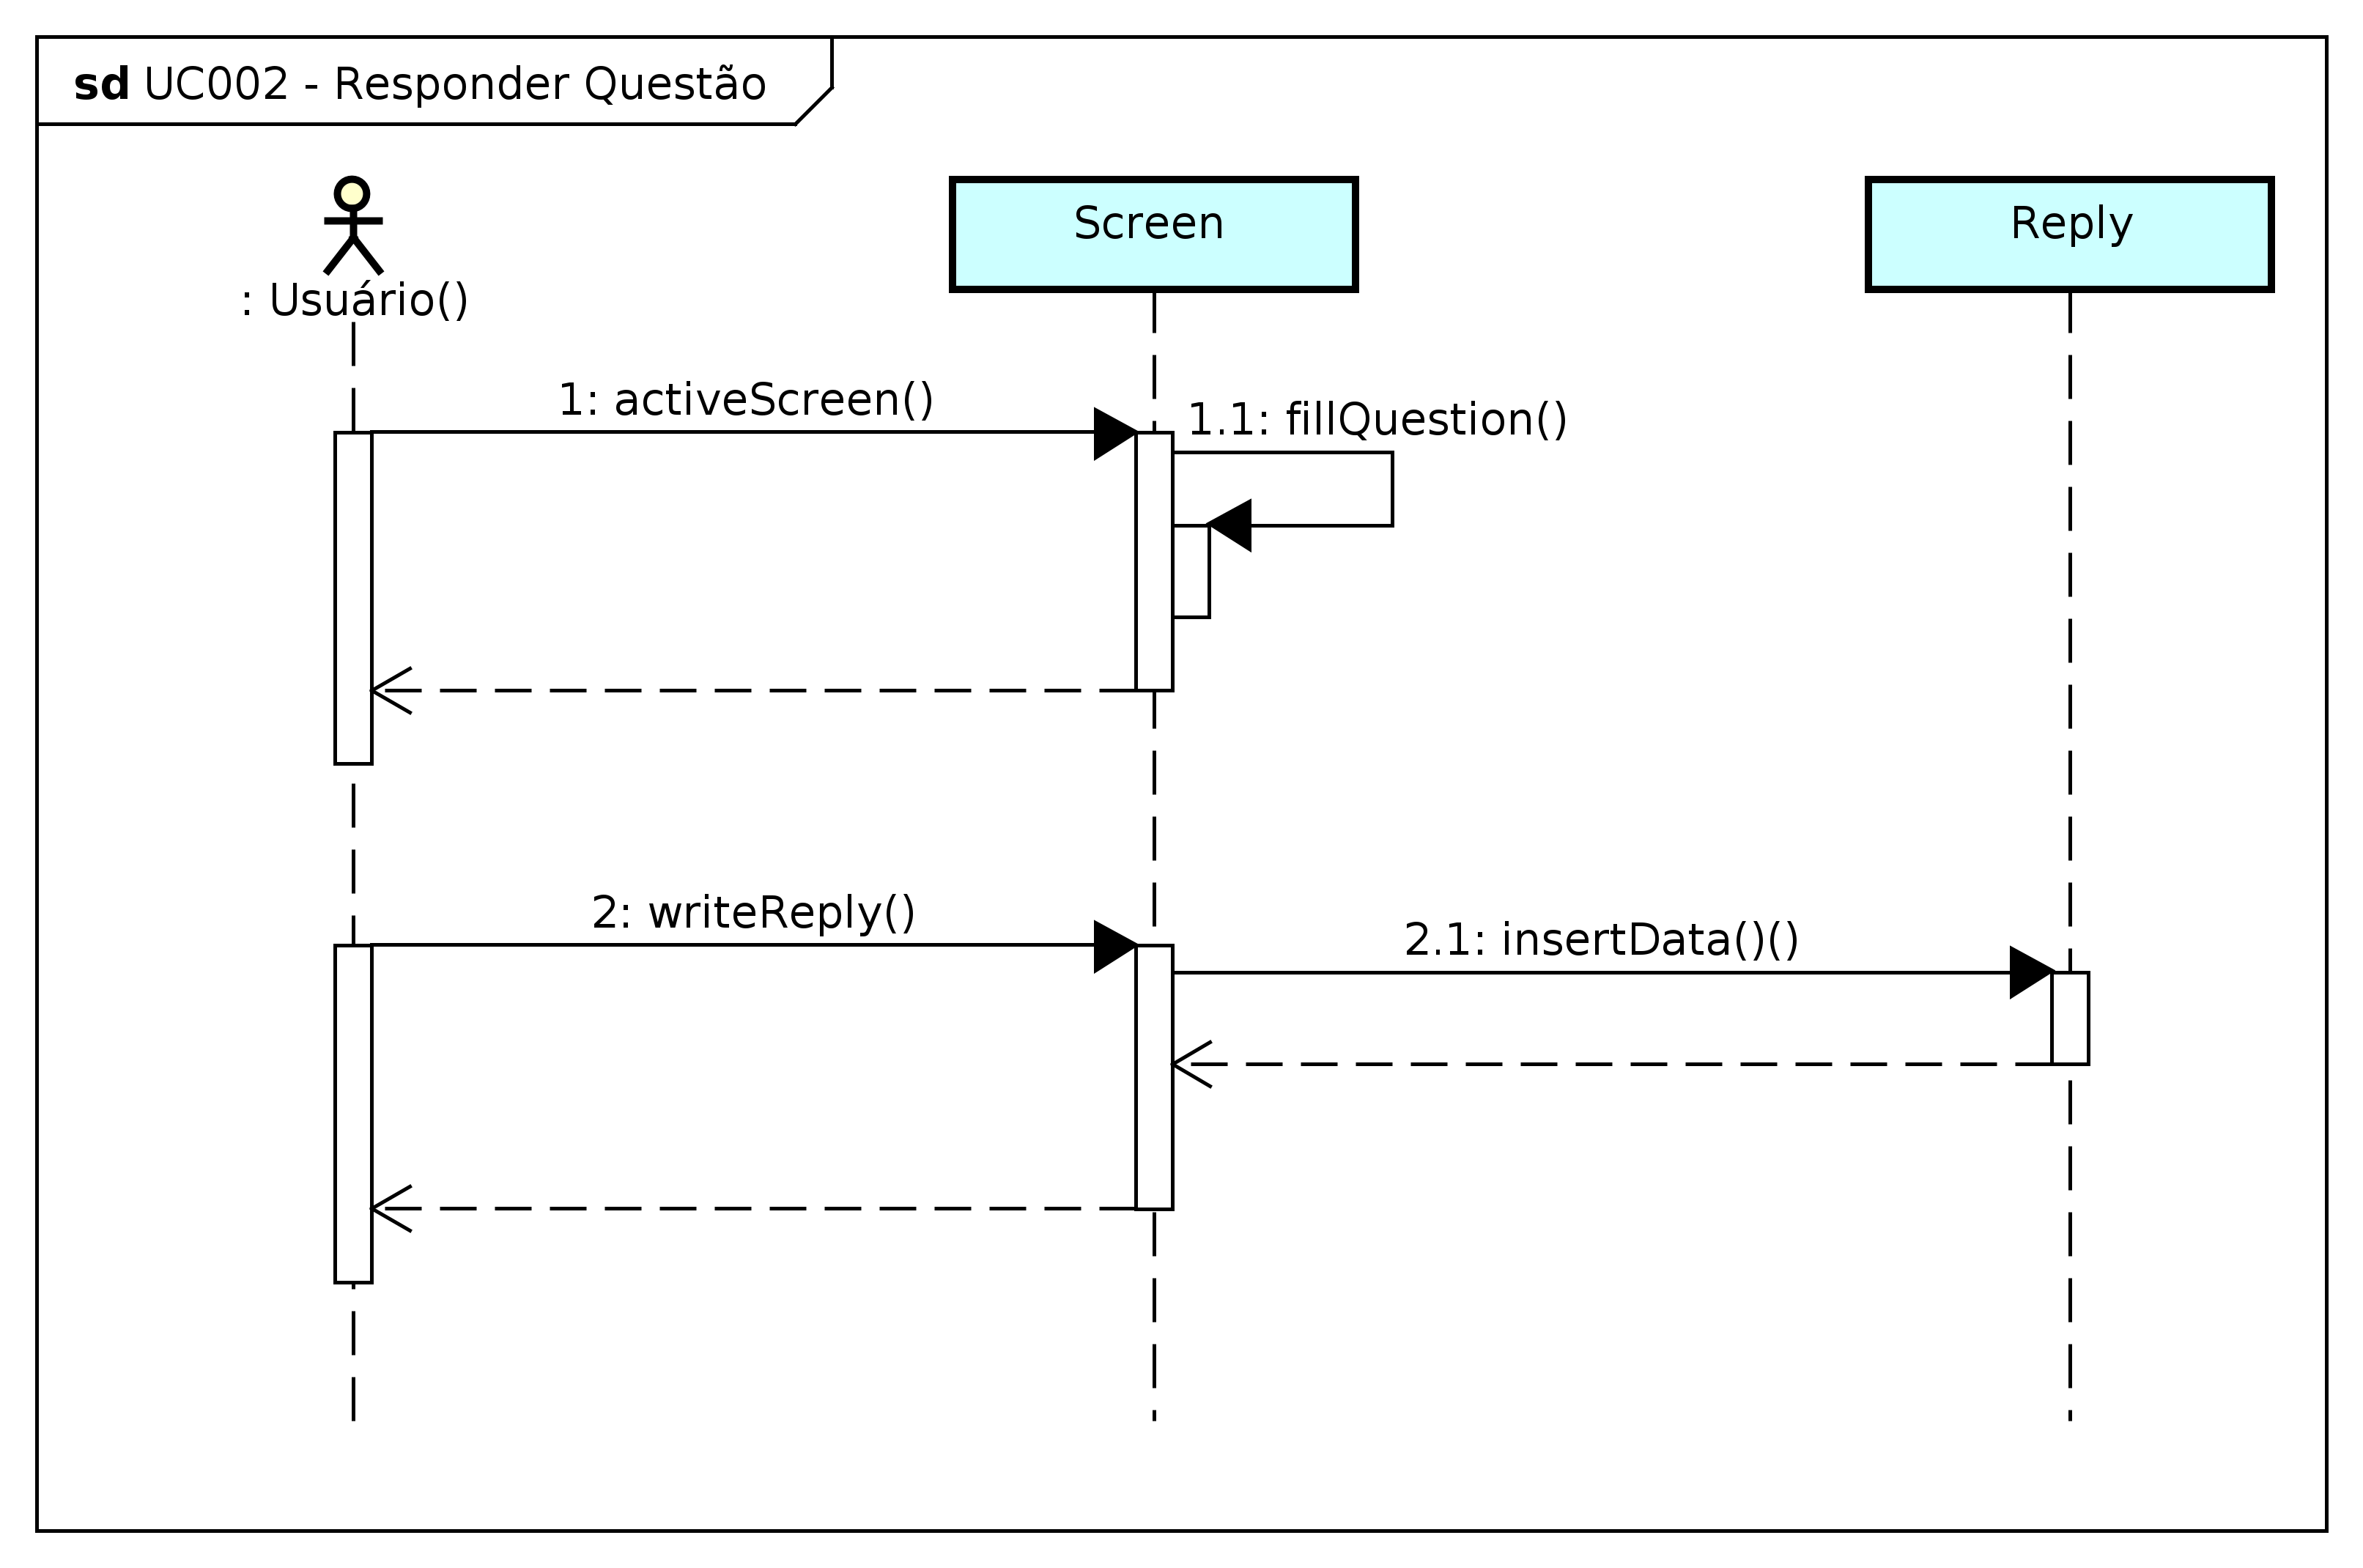
\includegraphics[width=16cm]{UC002-ResponderQuestao.png}
\caption{Diagrama de caso de uso UC002 - Responder Questão. Fonte: os autores.}
\label{fig:UC002}
\end{figure}

\begin{figure}[!htb]
\centering
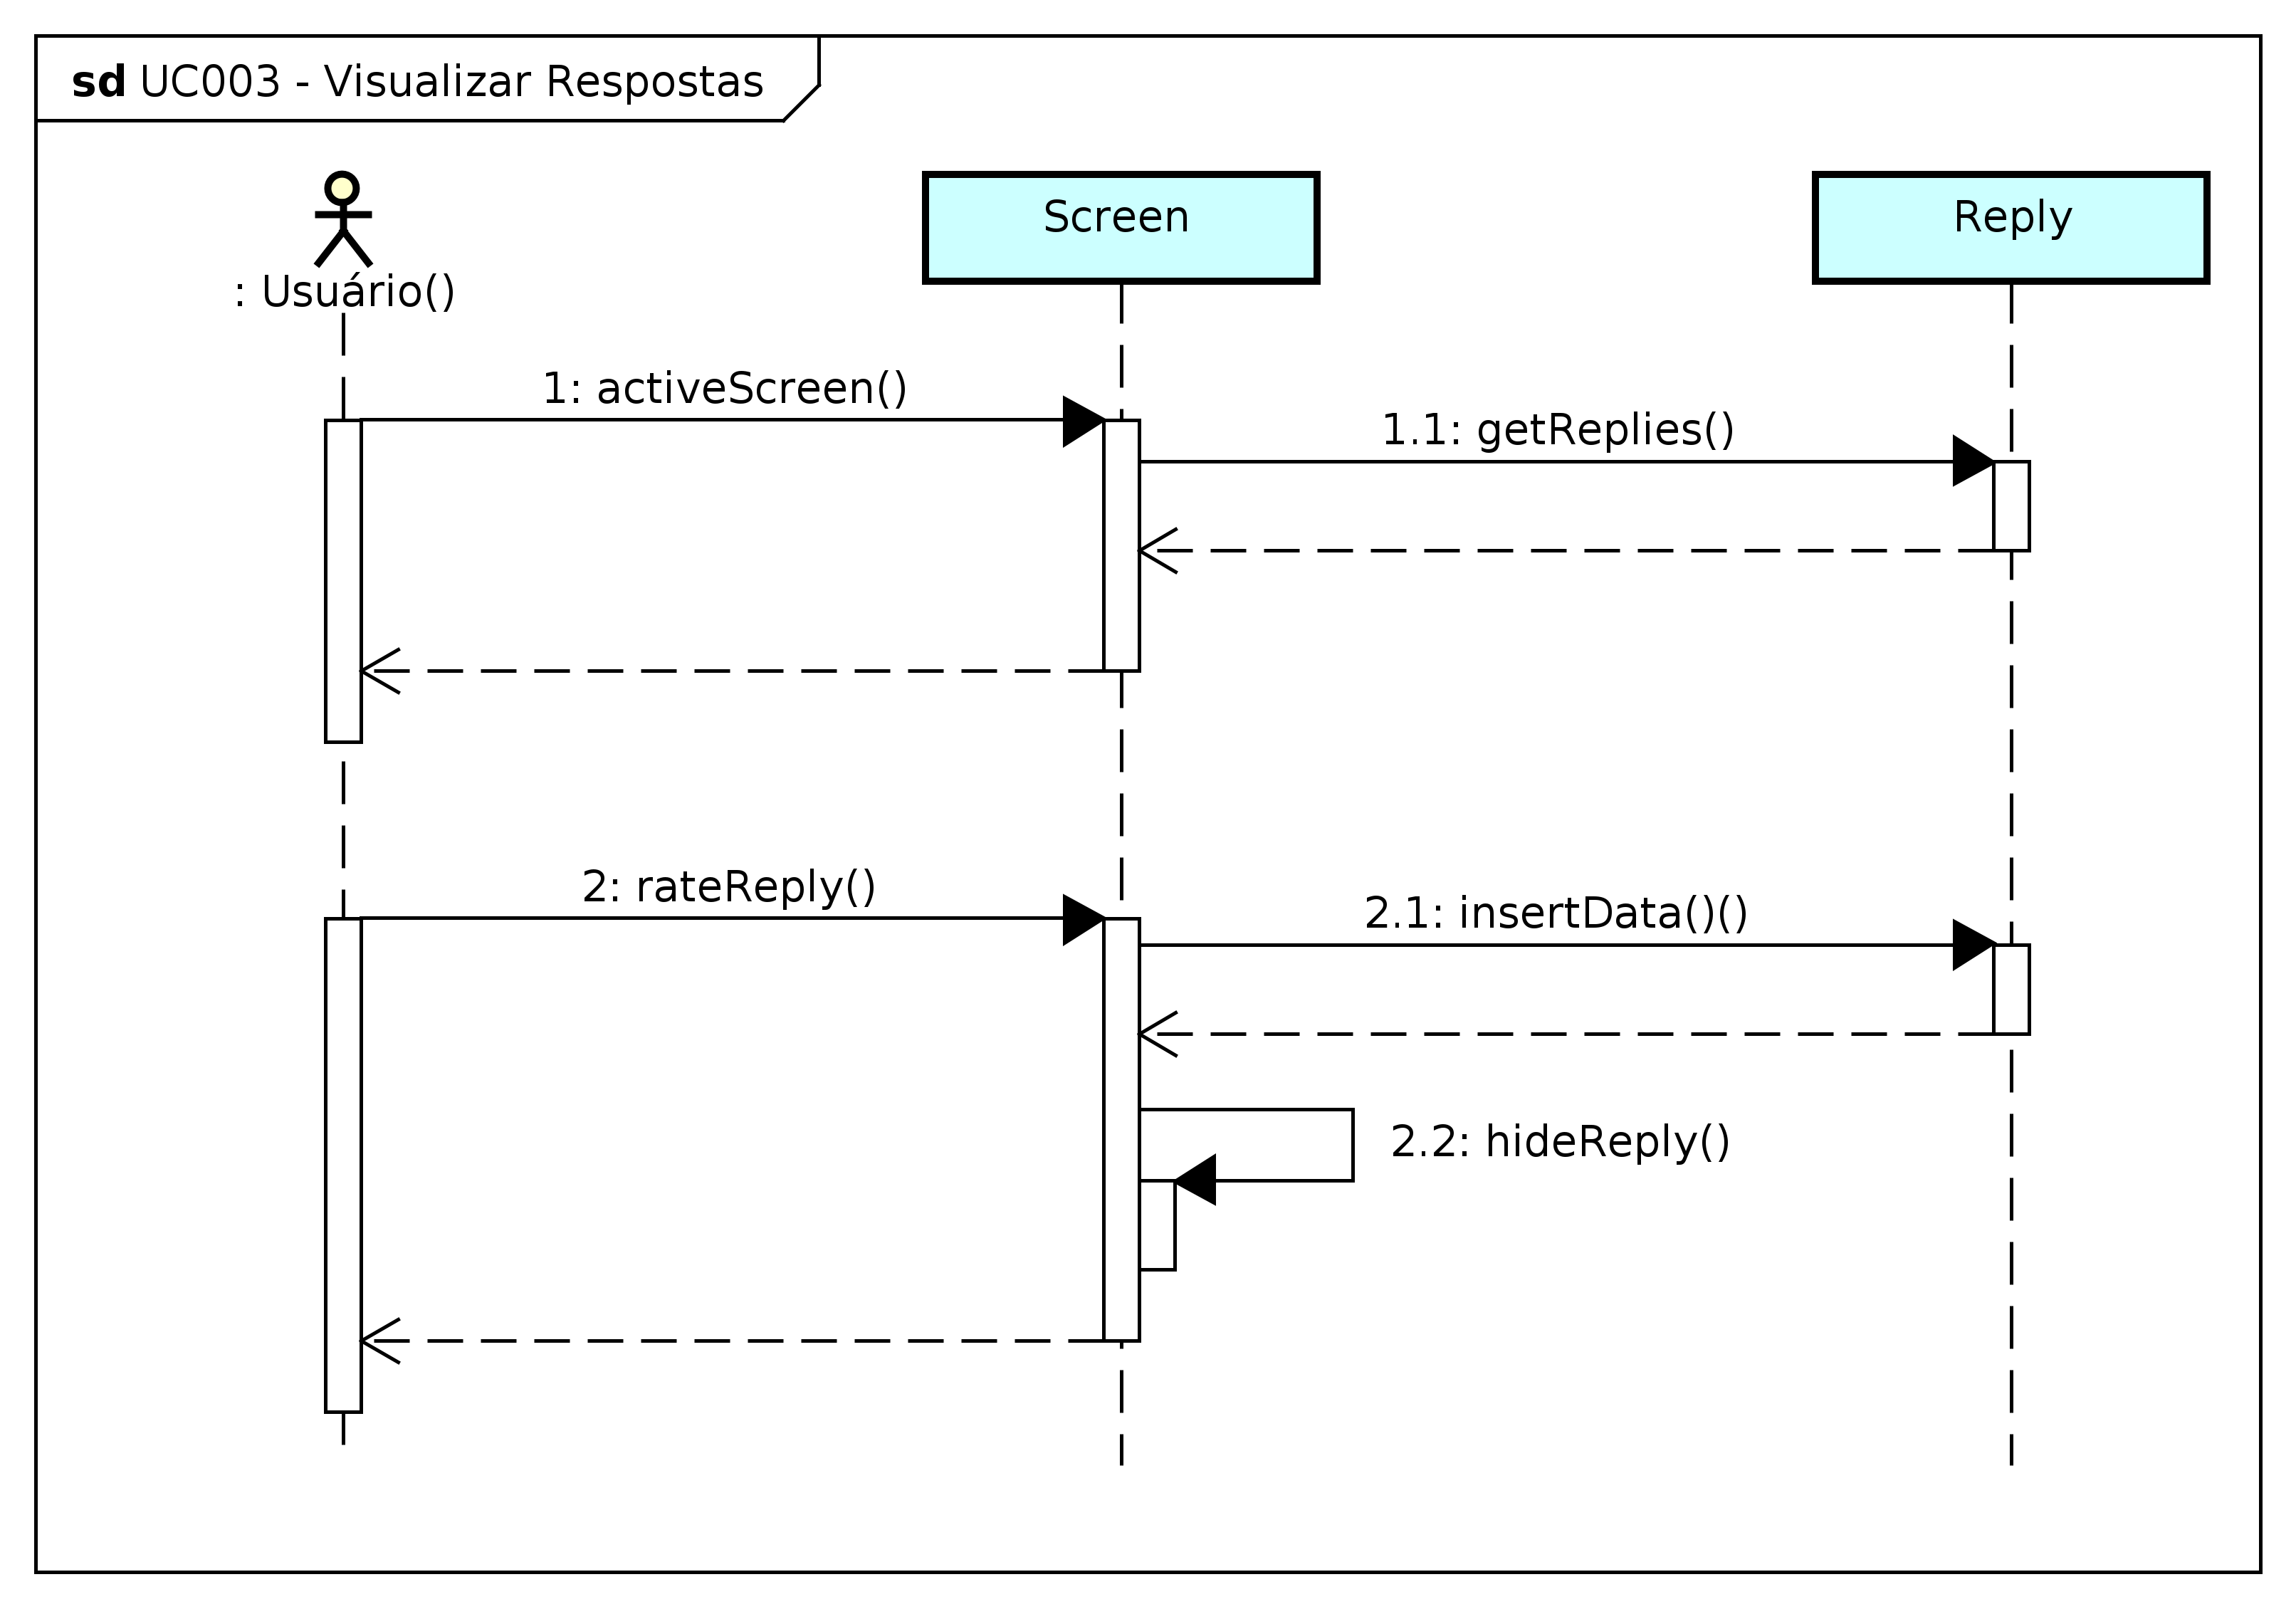
\includegraphics[width=16cm]{UC003-VisualizarRespostas.png}
\caption{Diagrama de caso de uso UC003 - Visualizar Respostas. Fonte: os autores.}
\label{fig:UC003}
\end{figure}

\begin{figure}[!htb]
\centering
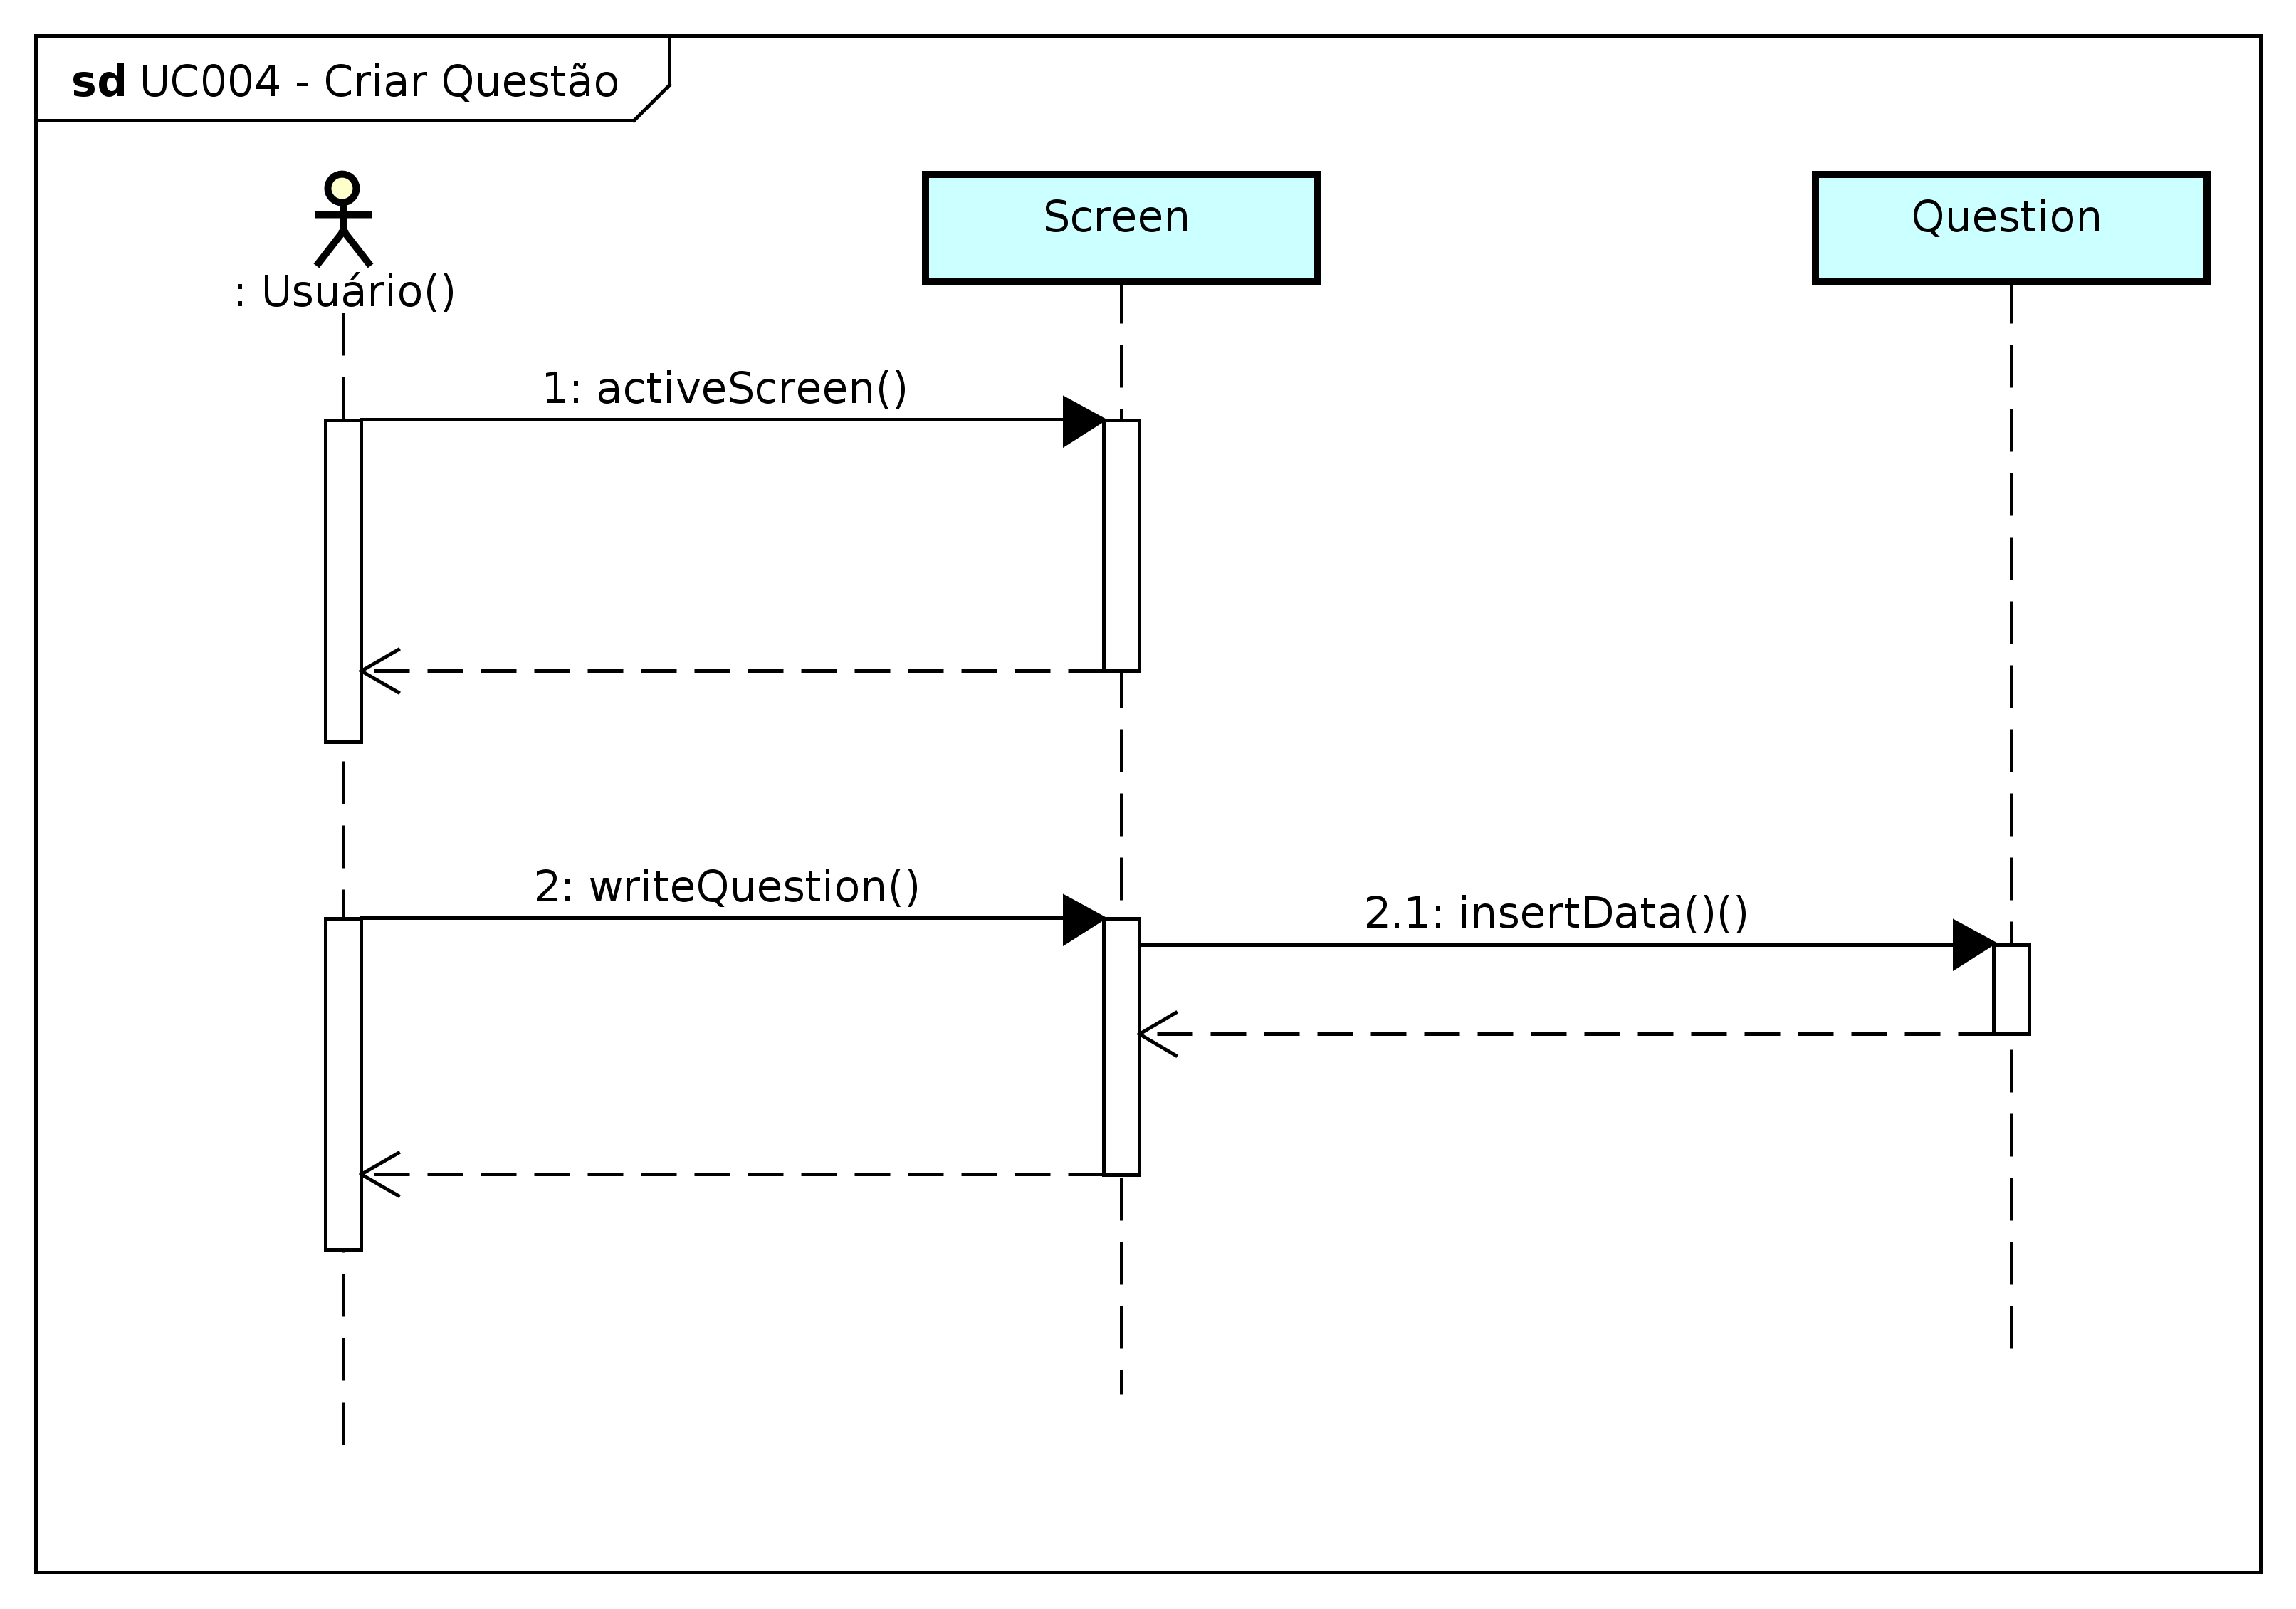
\includegraphics[width=16cm]{UC004-CriarQuestao.png}
\caption{Diagrama de caso de uso UC004 - Criar Questão. Fonte: os autores.}
\label{fig:UC004}
\end{figure}

\begin{figure}[!htb]
\centering
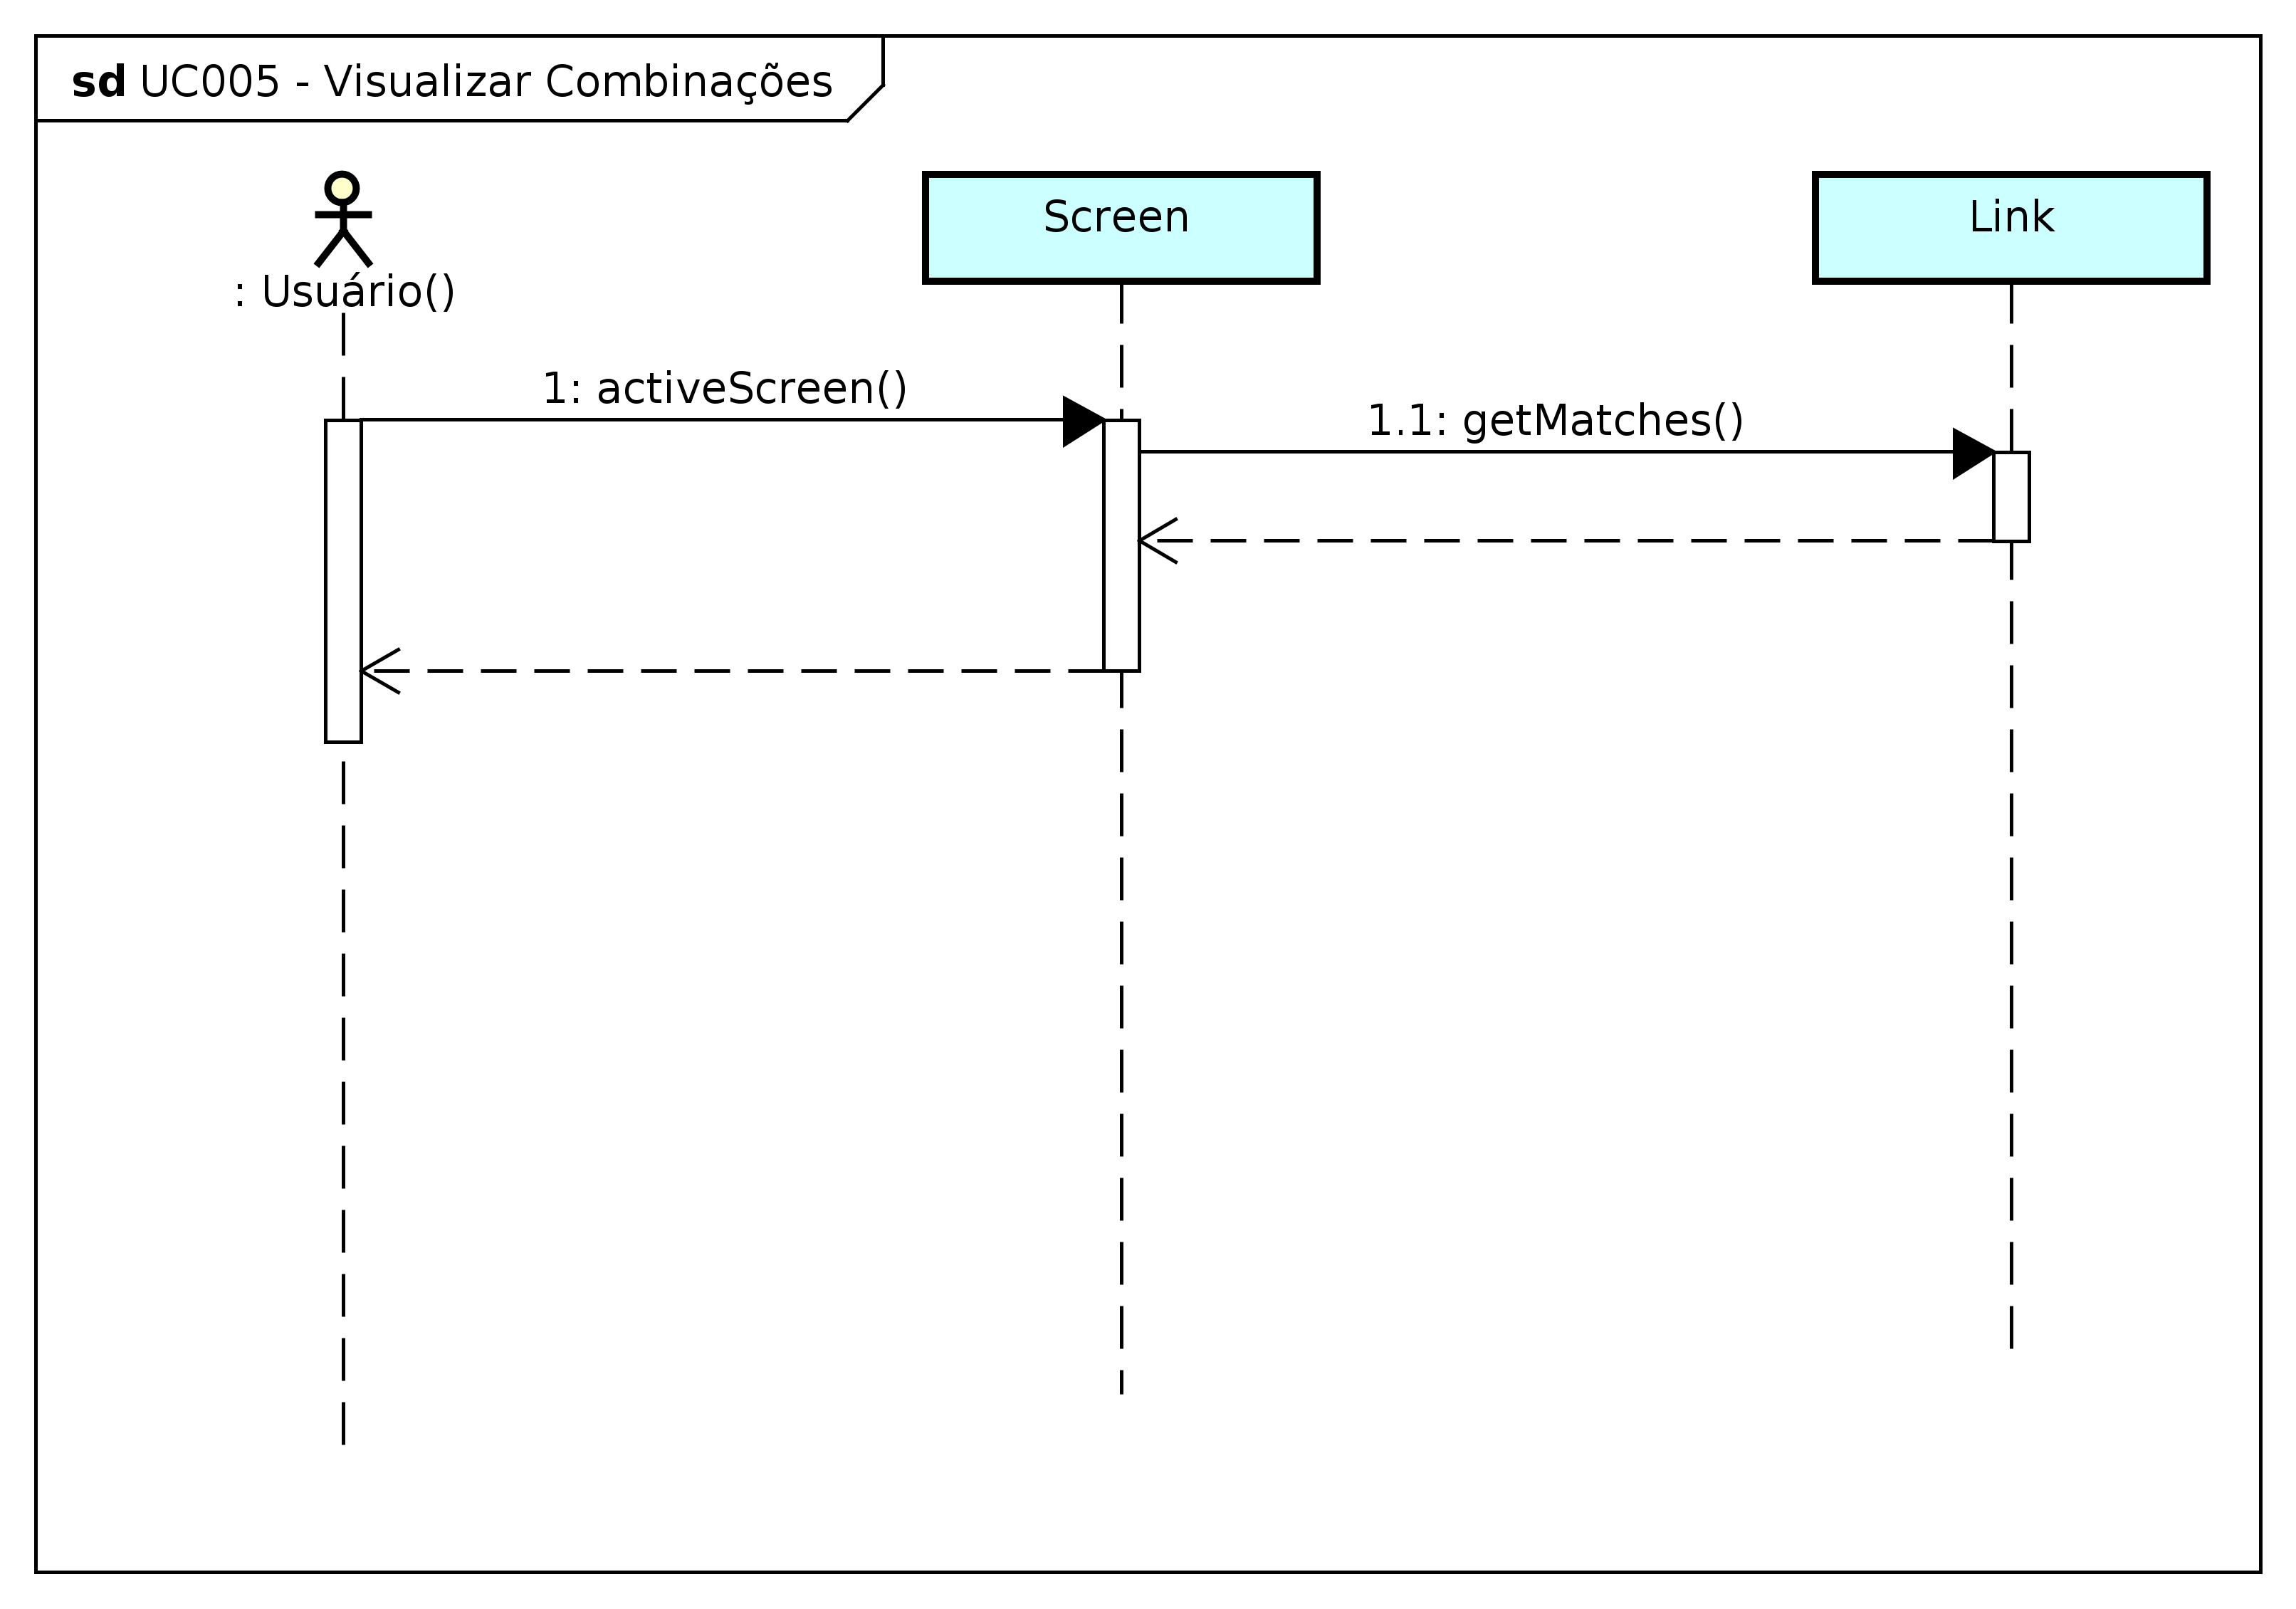
\includegraphics[width=16cm]{UC005-VisualizarCombinacoes.png}
\caption{Diagrama de caso de uso UC005 - Visualizar Combinações. Fonte: os autores.}
\label{fig:UC005}
\end{figure}

\section{Especificação de Casos de Uso}

\subsection*{UC001 - Visualizar Questões}

Descrição: Este caso de uso tem a função de apresentar as questões para o usuário como em um feed.
Data view: Figura \ref{fig:prot_perguntas} na página \pageref{fig:prot_perguntas}

Fluxo de eventos principal:

\begin{enumerate}

\item O sistema busca as questões mais recentes para o usuário logado.
\item O sistema carrega as questões buscadas.
\item O sistema apresenta a tela.
\item O usuário escolhe uma questão para responder.
\item O sistema chama UC002.

\end{enumerate}

\subsection*{UC002 - Responder Questão}

Descrição: Este caso de uso tem a função de apresentar os recursos envolvidos no processo de responder uma questão.

Data view: Figura \ref{fig:prot_escreverResposta} na página \pageref{fig:prot_escreverResposta}

Fluxo de eventos principal:

\begin{enumerate}

\item O sistema recebe a questão escolhida.
\item O sistema preenche o card com a questão escolhida.
\item O sistema apresenta a tela.
\item O usuário escreve uma resposta.
\item O usuário clica no botão "Enviar".
\item O sistema registra a resposta.

\end{enumerate}

\subsection*{UC003 - Visualizar Respostas}

Descrição: Este caso de uso tem a função de apresentar para o usuário as respostas que ele recebeu para as questões que criou.

Data view: Figura \ref{fig:prot_respostas} na página \pageref{fig:prot_respostas}

Fluxo de eventos principal:

\begin{enumerate}

\item O sistema busca respostas que ainda não foram avaliadas.
\item O sistema apresenta a tela.
\item O usuário escolhe e avalia uma resposta.
\item o sistema esconde a resposta avaliada.

\end{enumerate}

\subsection*{UC004 - Criar Questão}

Descrição: Este caso de uso tem a função de apresentar os recursos necessários para o processo de criação de questões.

Data view: Figura \ref{fig:prot_escreverPergunta} na página \pageref{fig:prot_escreverPergunta}

Fluxo de eventos principal:
\begin{enumerate}
\item O sistema apresenta a tela.
\item O usuário rescreve a questão. (E1)
\item O usuário clica no botão enviar.
\item O sistema registra a questão.
\end{enumerate}

Fluxo de eventos de exceção:

E1. A questão deve conter ao menos um caractere.

\begin{enumerate}
\item O sistema bloqueia o botão de enviar até que a condição seja satisfeita.
\end{enumerate}

\subsection*{UC005 - Visualizar Combinações}

Descrição: Este caso de uso tem a função de apresentar a lista de usuários que foram considerados potenciais amizades do usuário logado.

Data view: Figura \ref{fig:prot_conversas} na página \pageref{fig:prot_conversas}

Fluxo de eventos principal:
\begin{enumerate}
\item O sistema busca as combinações.
\item O sistema carrega as combinações.
\item o sistema apresenta a tela.
\item O usuário escolhe uma combinação. (E1)
\item Sistema apresenta o mensageiro instantâneo.
\end{enumerate}

Fluxo de eventos de exceção:

E1. O usuário não tem uma combinação.

\begin{enumerate}
\item Exibe a tela sem nenhum contato.
\end{enumerate}



